\documentclass[12pt]{article}
\usepackage[french]{varioref}
\usepackage[french]{babel}
\usepackage[T1]{fontenc}
\usepackage{lmodern}
\usepackage{graphicx}
\usepackage{float}
\usepackage{minted}
\usepackage{amsmath}
\begin{document}

\begin{titlepage}
      \vspace*{\stretch{1}}
      \begin{center}
            {\large\bfseries Rapport de projet \\[1ex]}
            {\LARGE\bfseries Continuation Projet \\[2ex]}
            {\huge\bfseries Bataille navale\\[6.5ex]}
            {\large\bfseries LEROY Florent\\[1ex]}
            \vspace{4ex}
            Rapport rédigé pour\\[5pt]
            \textit{Université de Rouen Normandie}\\[2cm]
            \textsc{\large Informatique}\\[12ex]
            \vfill
            Département d'informatique\\
            \vfill
            juin 2024
      \end{center}
      \vspace{\stretch{2}}
\end{titlepage}
\newpage
\tableofcontents
\newpage

\section{Introduction}
\subsection{Cahier des charges}

L'\textbf{objectif} de ce projet est de réaliser un programme possédant une
application graphique
permettant à un ou deux joueurs de jouer au jeu `Bataille navale'. Si un seul
joueur est présent, il pourra jouer contre une intelligence artificielle dont
il pourra choisir le niveau. Sinon, les deux joueurs pourront jouer en réseau.

\bigskip

L'exécutable devra être livré en format \texttt{.jar}. Et sera exécutable avec
un simple script shell pour éviter tous problèmes.

\bigskip

Le programme proposera les fonctionnalités suivantes :

\bigskip

\begin{itemize}
      \item[$\bullet$] Il sera possible de jouer contre un autre joueur,
            présent sur une autre machine (ou la même machine, en local). Dans
            ce cas-là,
            le programme utilisera le principe du modèle client-serveur afin de
            permettre à
            un joueur d'héberger la partie. Plus d'informations sur ce point
            seront
            disponibles dans la partie \textbf{Architecture réseau}.

            \bigskip

      \item[$\bullet$] Sinon, le joueur pourra jouer contre une intelligence
            artificielle avec trois niveaux de difficulté disponibles (Facile,
            moyen et
            Difficile). Plus d'informations sur le comportement de
            l'intelligence seront
            disponibles dans la partie \textbf{Intelligence artificielle}.
            \bigskip

      \item[$\bullet$] L'utilisation du programme se veut simple et intuitive.
            La manipulation des éléments graphiques se fera soit par simples
            clics sur des
            boutons, dans le cas du placement de bateaux sur la grille avant le
            début de la
            partie, la manipulation se fera par `drag-and-drop' des éléments
            graphiques sur
            une zone cible. Certaines actions complémentaires, cependant,
            pourront
            nécessiter l'utilisation du clavier. Plus d'informations se
            trouveront dans la
            partie \textbf{Utilisation de l'exécutable}.
\end{itemize}

\bigskip

Vis-à-vis des règles du jeu `Bataille navale', nous nous sommes basés sur les
règles du jeu `Touché-Coulé', commercialisé par Hasbro. Les règles sont :

\bigskip

\begin{itemize}
      \item[$\bullet$] Chaque joueur dispose d'une grille de dimension $10
                  \times 10$ –
            pouvant être numéroté de \textbf{1} à \textbf{10} dans la longueur
            et de
            \textbf{A} à \textbf{J} dans la largeur.

            \bigskip

      \item[$\bullet$] Chaque joueur pourra aussi disposer d'une grille
            supplémentaire
            afin
            de noter les tentatives d'attaques.

            \bigskip

      \item[$\bullet$] Chaque joueur dispose de 5 blocs ('bateaux') de
            largeur 1
            et de
            longueur différente :
            \begin{itemize}
                  \item[$\bullet$] 1 bateau de longueur 5
                  \item[$\bullet$] 1 bateau de longueur 4
                  \item[$\bullet$] 2 bateaux de longueurs 3
                  \item[$\bullet$] 1 bateau de longueur 2
            \end{itemize}

            \bigskip

      \item[$\bullet$] Un joueur ne peut voir la grille de son adversaire. Il
            voit
            seulement les endroits qu'il a touchés et le résultat de ces
            touches si c'est
            raté ou touché.

            \bigskip

      \item[$\bullet$] En début de partie, chaque joueur dispose ses bateaux.
            Dès que tous les blocs sont placés, la partie peut commencer. Les
            bateaux
            peuvent être placés n'importe où sur la grille, tant que ceux-ci ne
            sont pas ou
            n'ont pas une partie d'eux sur un autre bateau ou en-dehors de la
            grille.

            \bigskip

      \item[$\bullet$] Au tour par tour, un joueur va donner une coordonnée à
            l'adversaire. L'adversaire devra annoncer si, sur sa grille, la
            coordonnée
            contient une partie d'un bateau. S'ensuivent 3 scénarios :
            \begin{itemize}
                  \item[$\bullet$] La coordonnée ne continent pas de bateau.
                        Dans ce cas, l'adversaire déclarera \textbf{`Raté'}.
                  \item[$\bullet$] La coordonnée contient une partie d'un
                        bateau. Dans ce
                        cas,
                        l'adversaire déclarera \textbf{`Touché'}.
                  \item[$\bullet$] La coordonnée contient une partie d'un
                        bateau et
                        toutes les
                        autres parties dudit bateau ont déjà été touché.
                        Dans
                        ce cas, l'adversaire
                        déclarera \textbf{`Touché-coulé'}.
            \end{itemize}

            \bigskip

      \item[$\bullet$] À chaque tentative, le joueur devra noter sur sa grille
            auxiliaire
            le
            résultat du toucher.

            \bigskip

      \item[$\bullet$] La partie se termine dès lors que chaque bateau d'un des
            joueurs
            ait
            été \textbf{`touché-coulé'}. Dans ce cas, l'adversaire sera
            proclamé vainqueur.
\end{itemize}

\subsection{'Proof of concept'}

\begin{figure}[H]
      \centering
      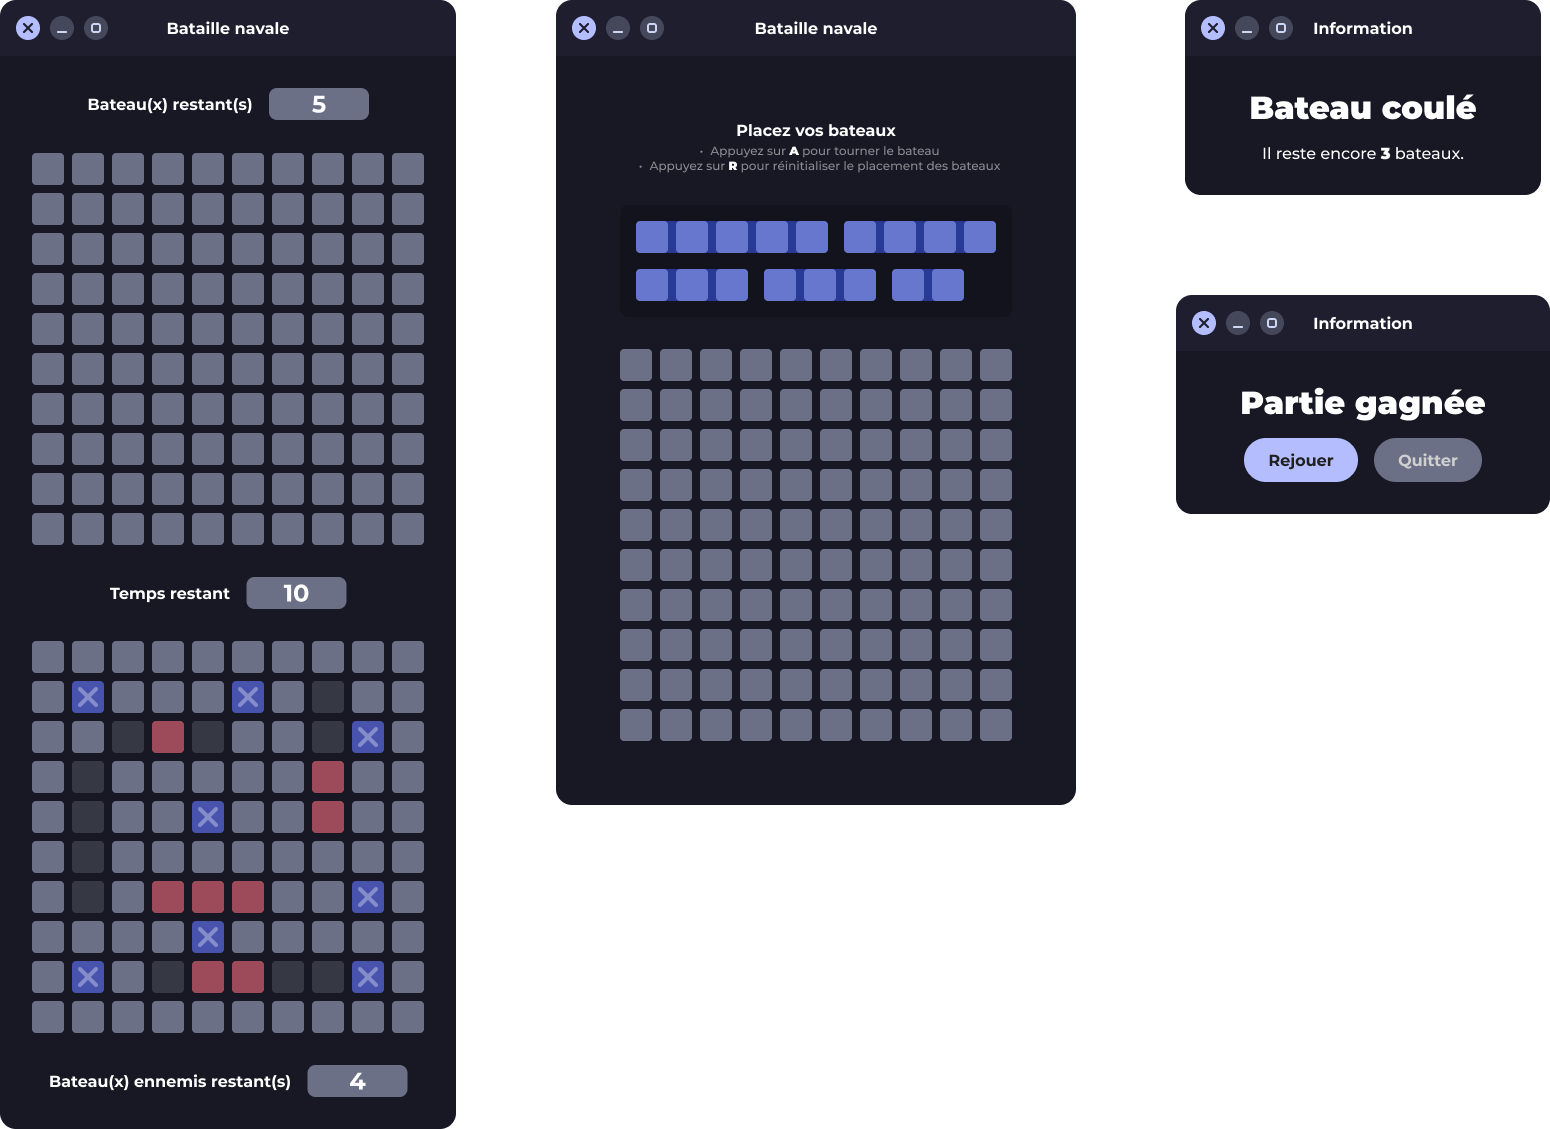
\includegraphics[width=0.75\linewidth]{images/POC.png}
      \caption{Concept de l'interface du jeu `Bataille navale'}
\end{figure}

De gauche à droite, et de haut en bas :
\begin{itemize}
      \item[$\bullet$] Interface en jeu contre un adversaire
      \item[$\bullet$] Interface de placement de bateaux
      \item[$\bullet$] Message d'indication en jeu
      \item[$\bullet$] Message de fin de partie
\end{itemize}

\bigskip

Cette maquette a été réalisée sous Figma, et a été créée avec des composants se
voulant issus des directives et des modules de la bibliothèque \\
GNOME/GTK4/LibAdwaita. La palette de couleur utilisée reprend la palette
Catppuccin Mocha.
Il s'agit seulement d'une vue d'artiste, n'ayant que pour objectif d'imaginer à
quoi pourrait ressembler l'interface.

\newpage

\section{Version initiale}
Ce projet étant la continuation du projet d'Application Informatique je vais
rapidement expliquer l'architecture du programme ainsi que les choix faits afin
de pouvoir mieux parler des modifications effectuées.

\bigskip

Le projet initiale dans un objectif d'utiliser un maximum les connaissances de
deuxième et troisième année a été programmé en java 1.7 et les interfaces
graphiques
sont réalisées en java swing. Le serveur lui est programmé en python, car il ne
travaille que sur des chaînes de caractères.

\bigskip

\subsection{Architecture du programme}
Dans le programme, il y a deux architectures à évoquer. L'architecture du code
en lui-même et l'architecture réseau, la manière dont est utilisé le serveur.
\bigskip
Pour expliquer l'architecture réseau, nous allons simuler un tour où le client
1 joue pour essayer de toucher un bateau du client 2.
\begin{figure}[H]
      \centering
      \includegraphics[width=\textwidth]{images/image BN initiale/BN initial
            Réseau.png}
      \caption{Diagramme fonctionnel de l'architecture réseau lors d'un tour.}
\end{figure}
\bigskip
Via le diagramme on voit que le serveur ne sert que de proxy en transmettant
simplement les informations d'un client vers un autre sans vérifier les
informations.
\begin{figure}[H]
      \centering
      \includegraphics[width=\textwidth]{images/image BN initiale/BN initial
            UML.png}
      \caption{Diagramme UML de la structure du programme}
\end{figure}
\bigskip
\subsection{Apparence de la version initiale}

\begin{figure}[H]
      \centering
      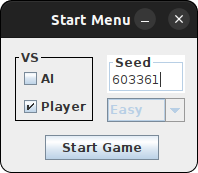
\includegraphics[width=0.33\linewidth]{images/image BN
            initiale/image.png}
      \caption{Écran de début de partie}
\end{figure}
\begin{figure}[H]
      \minipage{0.48\textwidth}
      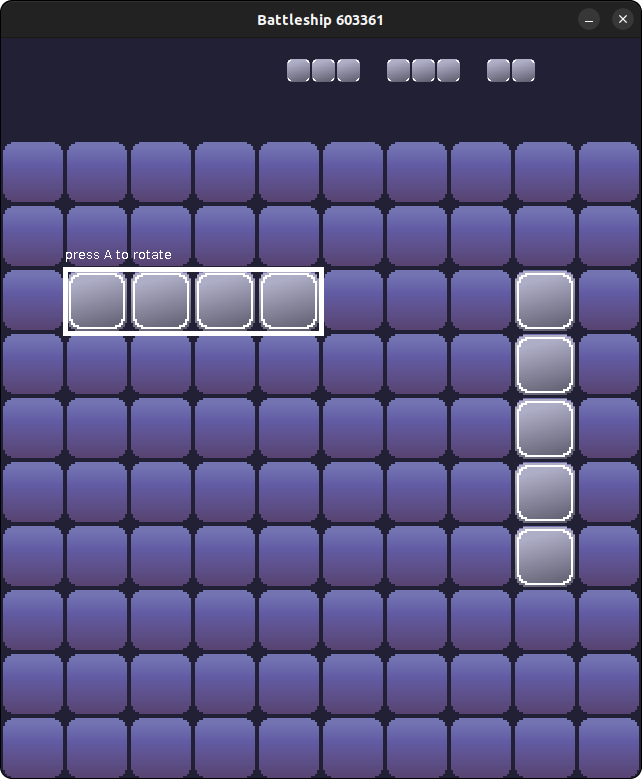
\includegraphics[width=\linewidth]{images/image BN
            initiale/image2.png}
      \caption{Écran de placement des bateaux}
      \endminipage\hfill
      \minipage{0.48\textwidth}
      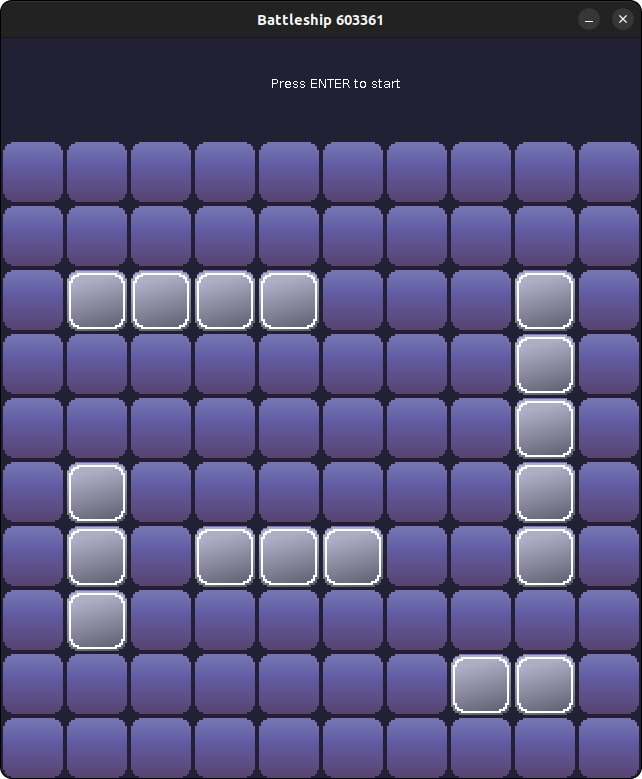
\includegraphics[width=\linewidth]{images/image BN
            initiale/image3.png}
      \caption{Écran de placement des bateaux (après avoir placé tous les
            bateaux)}
      \endminipage\hfill
\end{figure}

\begin{figure}[H]
      \minipage{0.48\textwidth}
      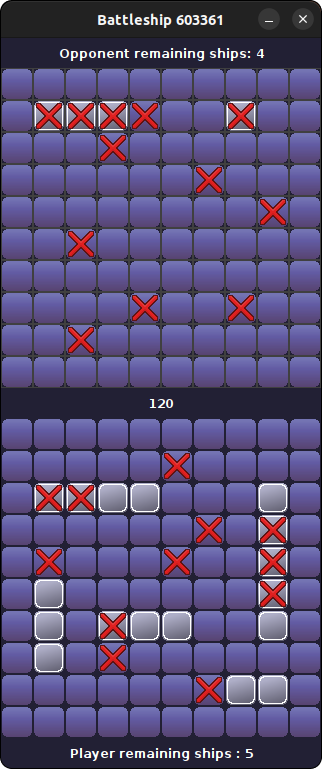
\includegraphics[width=\linewidth]{images/image BN
            initiale/image4.png}
      \caption{Écran de partie (avec un autre joueur en
            ligne)}
      \endminipage\hfill
      \minipage{0.48\textwidth}
      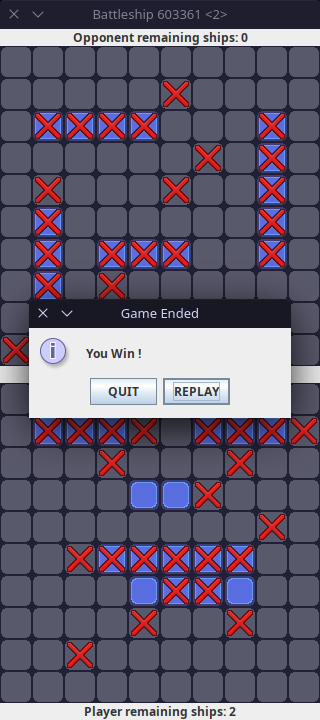
\includegraphics[width=\linewidth]{images/image BN
            initiale/image5.png}
      \caption{Écran de fin de partie}
      \endminipage\hfill
\end{figure}

\subsection{Intelligence artificielle}

L'implémentation de l'intelligence artificielle n'ayant pas été modifiée par
rapport à la version initiale. Cette partie est à but de rappeler.

Afin de permettre à un joueur de jouer en absence d'adversaire humain ou en
absence de connexion, nous avons implanté un ensemble d'algorithmes permettant
de simuler le comportement d'un joueur.
\subsubsection{Implémentations}
Du point de vue de l'implémentation, la classe responsable de représenter et de
permettre une interaction avec l'intelligence artificielle se nomme
\texttt{AIPlayer}, et se présente comme une couche entre \texttt{GamePanel} et
\texttt{Game} où s'effectue l'action de l'IA\@.

Ces méthodes permettent d'annoncer à la machine adverse où elle a été touchée,
de toucher le joueur selon des coordonnées (voir ci-dessous), et de l'informer
en retour si le tir a réussi ou pas.

Le plus grand du travail est réalisé par les classes réalisant la
classe abstraite \texttt{AIModel}. Ces classes réalisent la méthode
\texttt{chooseCoordinates ()} qui choisit de manière méthodique (ou non)
l'emplacement du prochain coup.
\bigskip

\subsubsection{Algorithmes}
Dans notre implémentation actuelle, il existe 3 modèles d'IA différents,
classés selon leur niveau de difficulté :

\bigskip

\begin{itemize}
      \item[$\bullet$] \texttt{StupidAI} représente l'IA de difficulté facile.
            Son
            comportement est relativement simple : à chaque tour, l'IA récupère
            les
            coordonnées de toutes les cases non touchées et choisit une
            coordonnée au
            hasard.

            \bigskip

      \item[$\bullet$] \texttt{AdvancedAI} représente l'IA de difficulté
            difficile. Son comportement est, lui aussi, relativement simple : à
            chaque
            tour, l'IA récupère les coordonnées de toutes les cases non
            touchées, et les
            coordonnées des cases autour des points touchés et réussi (nommés
            `touchées'
            dans les règles du jeu), puis choisis en priorité les cases
            adjacentes aux
            coups réussis, si ces cases n'existent pas, il choisit une
            coordonnée au hasard
            sinon, revenant donc au comportement de l'IA de difficulté facile.

            \bigskip

      \item[$\bullet$] \texttt{ChoosyAI} représente l'IA de difficulté
            intermédiaire. Son
            comportement est un mélange des comportements des deux IA indiqués
            ci-dessus,
            la seule différence résidant dans le fait que l'IA peut choisir
            soit une case
            au hasard avec une chance de $\frac{2}{5}$, soit une case
            adjacente, avec une
            chance de $\frac{3}{5}$. Deux macroconstantes peut être utilisée
            pour modifier
            ces probabilités.
\end{itemize}
\subsubsection{Améliorations possibles}
Il existe plusieurs moyens pour rendre l'intelligence artificielle plus
efficace, et donc plus dure.
\bigskip
\begin{itemize}
      \item[$\bullet$] Pour accélérer le repérage des bateaux, nous pouvons
            procéder avec
            un
            motif en carreaux, comme suit :
            \[
                  \begin{bmatrix}
                          & X &   \\
                        X &   & X \\
                          & X &   \\
                  \end{bmatrix}
            \]
            Sachant qu'un bateau est de longueur minimum 2, cela signifie
            que
            l'on peut
            trouver au moins une des cases du bateau, quelque soit son
            emplacement.

            \bigskip
            $
                  \begin{bmatrix}
                          & X &   \\
                        X &   & O \\
                          & X & O \\
                  \end{bmatrix}
            $
            $
                  \begin{bmatrix}
                          & O &   \\
                        X & O & X \\
                          & X &   \\
                  \end{bmatrix}
            $
            $
                  \begin{bmatrix}
                        O & O &   \\
                        X &   & X \\
                          & X &   \\
                  \end{bmatrix}
            $
            $
                  \begin{bmatrix}
                          & X &   \\
                        X &   & X \\
                        O & O &   \\
                  \end{bmatrix}
            $
            $\ldots$

            \bigskip

            Cela signifie aussi que le nombre de cases potentiellement
            touchables sont au plus divisées par 2, rendant l'IA bien plus
            redoutable. Une
            fois un bateau trouvé, le comportement ne changera pas.

            \bigskip

      \item[$\bullet$] Une des variables potentiellement accessible à l'IA
            pouvant avoir
            une
            influence sur son comportement est le nombre de bateaux restant, et
            surtout sa
            variation après avoir touché un bateau. Cela pourrait indiquer à
            l'intelligence
            artificielle qu'il faut qu'elle arrête de chercher autour de ce
            bateau, car
            celui-ci a déjà été touché-coulé.

            \bigskip

            Nous pouvons remarquer que cette amélioration n'augmente pas
            réellement la
            difficulté de l'intelligence artificielle, sachant que ce
            comportement est
            assimilable à l'action de chercher des cases adjacentes aux bateaux
            déjà
            touchés.

            \bigskip
\end{itemize}
\subsubsection{Placement des bateaux}
Pour permettre à l'IA de placer des bateaux sans intervention humaine, elle
utilise la classe \texttt{ShipPlacer}, lui permettant de placer les bateaux de
manière complètement aléatoire, et donc impossible à prédire par le joueur
humain adverse. Cela se fait par l'appel à la méthode \texttt{placeShips ()}.

\bigskip

Pour ce faire, chaque bateau est placé dans l'ordre de génération (voir la
méthode \texttt{generateShips ()}), avec une coordonnée de départ et une
orientation (horizontale ou verticale) aléatoire. L'algorithme utilisé est de
type glouton/brute force, c'est-à-dire que le prochain bateau ne sera placé
qu'une fois que le bateau précédent a trouvé un emplacement adéquat, à savoir
un emplacement ne dépassant pas de la grille et non occupé par un autre bateau.

\bigskip

Deux remarques sont à faire sur cet algorithme.

\bigskip

Tout d'abord, on peut se poser la question sur le temps d'exécution de cette
méthode, voire sa complexité. En effet, la capacité de l'algorithme à se
terminer dépend des nombres aléatoires tirés et du placement des bateaux
précédents, donc sa complexité et son temps d'exécution est grandement
variable.

\bigskip

Nous pouvons au moins assurer la capacité de l'algorithme à atteindre la fin.
En effet, il n'existe, à notre connaissance, aucun placement de $n-1$ bateaux
(ici, $n$ = 5) sur une grille de 10$\times$10 (à savoir la grille utilisée pour
la
modélisation du jeu) qui empêcherait le placement du $n^e$ bateau, la grille
proposant toujours suffisamment de cases et d'emplacements de taille maximum 5
pour placer le dernier bateau, quelle que soit sa taille.

\bigskip

La seconde remarque tient sur le fait que, malgré la capacité de l'algorithme à
placer chaque bateau avec succès, quels que soient les nombres aléatoires
tirés, la taille des bateaux et la relative petitesse de la grille peut forcer
l'algorithme à toujours placer ses bateaux dans la même orientation, ce point
étant à ce jour le seul comportement à peu près prévisible venant du placement
des bateaux.

\newpage

\section{Nouvelle Version}

Cette nouvelle version du projet a pour but d'appliquer les améliorations
possibles que nous avons constatées pour le projet initial. Et aussi d'utiliser
des outils récents pour le réaliser. C'est pour cette raison que cette version
du projet a été programmée en utilisant Java 21 ainsi que JavaFX 21 et FXML
pour les interfaces graphiques.

Pour cette nouvelle version j'ai aussi utilisé un gestionnaire de dépendance
\texttt{Maven}. Cela a pour principal avantage que, par exemple moi et mon
professeur référent n'utilisons pas le même IDE mais grâce à Maven nous n'avons
pas eu de problème de compatibilités car Maven permet de gérer ce genre de
chose.

\bigskip

\subsection{Architecture du code coté client}
\begin{figure}[H]
      \centering
      \includegraphics[width=\textwidth]{images/image BN V2/Diagramme UML
            V2.png}
      \caption{Diagramme UML architecture code coté client}
\end{figure}
\bigskip
Maintenant, nous allons rentrer un peu plus dans le détail de chaque classe ou
module afin de mieux expliquer le fonctionnement du programme.

\bigskip

\subsubsection{Module \texttt{Ship}}

Le module \texttt{Ship} représente les bateaux, il sert de modèle à la classe
graphique utilisé pour la représentation et la manipulation via `drag-and-drop'
dans la classe \texttt{GraphicShip}. Il a pour but de retenir le type de
chaque bateau (sa taille) ainsi que les coordonnées sur lesquelles il est
positionné. La classe \texttt{Ship} n'est composée que de deux éléments :
\begin{itemize}
      \item[$\bullet$] Sa longueur : la taille en nombre de cases occupées par
            le bateau.
            Taille passée en paramètre au constructeur lors de l'instanciation
            d'un nouveau
            bateau.
            \bigskip
      \item[$\bullet$] Ses coordonnées : une liste de \texttt{Point2D}
            contenant
            les
            coordonnées
            de chaque case occupée par le bateau.
\end{itemize}

\bigskip

\subsubsection{Classe \texttt{TileState}}

La classe \texttt{TileState} est une classe énumérée représentant toutes les
valeurs que peut avoir une case de la grille de bataille navale.

\bigskip

\subsubsection{Module \texttt{Grid}}

Le module \texttt{Grid} simule le comportement d'une grille de bataille navale.
Lors de l'instanciation d'une grille, on lui donne en paramètre un tableau de
\texttt{Ship} afin que la grille ait connaissance de l'emplacement de chaque
bateau. Dans ce module, il y a une méthode principale :
\begin{minted}[bgcolor=lightgray, tabsize=2, fontsize=\small]{java}
      void hit (int row, int col);
\end{minted}
Elle simule un tir sur la case de ligne \texttt{row} et colonne
\texttt{col} cette fonction peut renvoie une exception
\texttt{PropertyVetoException} si la condition associée au
\texttt{VetoableChangeSupport} sur la propriété \texttt{PROP\_GRID} via la
fonction
\texttt{addVetoableChangeListener} n'est pas respectée.

\bigskip

La méthode
\begin{minted}[bgcolor=lightgray, tabsize=2, fontsize=\small]{java}
      List<List<Point2D>> getShip ();
\end{minted}
renvoie une liste où chaque élément de cette liste
est une liste contenant les coordonnées des cases occupées par un bateau.
Lorsqu'une case occupée par un bateau est touchée, on retire cet élément de la
liste associée au bateau lorsque la liste associée à un bateau est vide cela
veut dire que le bateau est entièrement détruit donc nous retirons cette liste
de la liste contenant les bateaux. Ainsi, si la liste est vide alors tous les
bateaux de la grille ont été détruits. C'est pour cette raison qu'à chaque fois
que l'on touche un bateau, on doit recalculer la liste des bateaux.

\bigskip

Les attributs statiques de type \texttt{String} dans l'interface \texttt{Grid}
sont les noms des propriétés auxquelles on ajoutera des écouteurs qui seront
notifiés à chaque modification de la valeur associée afin d'actualiser
l'interface graphique.

\bigskip

\subsubsection{GamePanel}

La classe \texttt{GamePanel} s'occupe de la simulation de la partie du côté du
joueur, elle gère donc la grille du joueur qui est une instance de
\texttt{Grid} ainsi que la version `cache' de la grille de l'adversaire. Cette
version `cache' de la grille de l'adversaire est la manière dont le joueur voit
la grille son adversaire. Au début de la partie, elle est vide, lorsque le
joueur tape l'ennemi, il voit sur cette version si la case sur laquelle il a
tiré est `touchée' ou `ratée'. Il possède aussi un attribut représentant le
nombre de bateaux restant à son adversaire.
\bigskip
Tous comme le module \texttt{Grid} le module \texttt{GamePanel} possède des
attributs statiques de type \texttt{String} qui les noms des propriétés
auxquelles on ajoutera des écouteurs qui seront notifiés à chaque modification
de la valeur associée.
\bigskip
Le module \texttt{GamePanel} possède deux méthodes principales :
\begin{minted}[bgcolor=lightgray, tabsize=2, fontsize=\small]{java}
      void playerHitEnnemy (int row, int col, TileState value);
      TileState ennemyHitPlayer (int row, int col);
\end{minted}
\begin{itemize}
      \item[$\bullet$] \texttt{playerHitEnnemy} met à jour la version `cache'
            de la grille
            adverse en mettant la case de ligne \texttt{row} et colonne
            \texttt{col} à la valeur passer en paramètre.
            \bigskip
      \item[$\bullet$] \texttt{ennemyHitPlayer} tire sur la grille du joueur à
            la case de
            ligne \texttt{row} et colonne \texttt{col} et renvoie le nouvel
            état de la case touchée.
\end{itemize}

\bigskip

\subsubsection{BNClient}

Gère la connexion avec le serveur ainsi que l'envoi des données et la réception
de celle-ci. Afin d'en faire un module pouvant être facilement réutilisé juste
en modifier la valeur des deux attributs statiques, il est considéré que le
module ne connaît pas le protocole de communication avec le serveur et que
seuls les modules utilisant \texttt{BNClient} en ont connaissance.

\bigskip

\subsubsection{Game}

La classe Game est la classe mère dans deux autres classe \texttt{GameVsPlayer}
et \texttt{GameVsIA}. Elle regroupe les attributs ainsi que les méthodes
communes aux deux autres classes.

\bigskip

\begin{minted}[bgcolor=lightgray, tabsize=2, fontsize=\small]{java}
      void hit (int row, int col)
\end{minted}
\begin{itemize}
      \item[$\bullet$] La méthode \texttt{hit} a pour but d'être appelé par
            l'interface graphique lors du tour de joueur, signifie que le
            joueur essaye de
            toucher la case de ligne row et colonne col. L'implémentation de
            cela dépend
            uniquement de si la partie est contre un joueur ou une IA, mais,
            reste
            similaire dans le principe.
\end{itemize}
\bigskip
\begin{minted}[bgcolor=lightgray, tabsize=2, fontsize=\small]{java}
      void getHit ()
\end{minted}
\begin{itemize}
      \item[$\bullet$] La méthode \texttt{getHit} est la version inverse de
            \texttt{hit}.
            Elle est appelée lorsque c'est le tour de l'adversaire et que le
            joueur attend
            que l'on lui dise quelle case est touché. Cette méthode est
            structurellement très différente selon le mode de jeux chaque, ces
            différences
            seront expliquées dans les parties ci-dessous consacrées à chaque
            type de partie.
\end{itemize}
\bigskip
\begin{minted}[bgcolor=lightgray, tabsize=2, fontsize=\small]{java}
      void run ()
\end{minted}
\begin{itemize}
      \item[$\bullet$] La méthode \texttt{run} s'occupe de la gestion du timer
            lors d'un tour de la partie. La méthode pour annoncer le changement
            de tour
            diffère selon le mode de jeu, mais reste très similaire.
\end{itemize}

\subsubsection{GameVsPlayer}
Cette classe a pour but de gérer la partie cotée joueur lorsque que la partie
est contre un autre joueur. Elle doit donc gérer toute la partie connexions au
serveur, envoie des messages ainsi que la réception des messages du serveur et
le traitement desdits messages (message d'erreur, réponse du serveur, arrêt de
la connexion).
\bigskip
\begin{minted}[bgcolor=lightgray, tabsize=2, fontsize=\small]{java}
      void getHit ()
\end{minted}
\begin{itemize}
      \item[$\bullet$] La méthode \texttt{getHit} dans la partie contre un
            joueur ne fait
            qu'attendre que le serveur lui dise quelle case est touché et
            quelle est la valeur de cette case. Et met à jour le modèle client
            ainsi que l'interface graphique en fonction des informations
            reçues.
\end{itemize}

\subsubsection{GameVsIA}
Cette classe gère la partie contre l'intelligence artificielle. Les écoutent et
envoie sur le serveur sont remplacées par des appels aux fonctions du modèle de
l'IA\@.
\bigskip
\begin{minted}[bgcolor=lightgray, tabsize=2, fontsize=\small]{java}
      void getHit ()
\end{minted}
\begin{itemize}
      \item[$\bullet$] Contrairement à lorsque que la partie est contre un
            joueur, ici,
            c'est le programme client qui effectue les calcules et
            vérifications de si une case peut être touché et quelle est la
            valeur de cette nouvelle case. Puis communique avec l'intelligence
            artificielle sur les résultats de ses calculs.
\end{itemize}
\bigskip
\begin{minted}[bgcolor=lightgray, tabsize=2, fontsize=\small]{java}
      void run ()
\end{minted}
\begin{itemize}
      \item Contre une IA la méthode \texttt{run} gère aussi le système de tour
            par tour, c'est elle qui dit au joueur et l'IA s'ils doivent jouer
            ou non.
\end{itemize}

\subsection{Architecture réseau}
Afin d'expliquer l'architecture réseau de cette nouvelle version, nous allons
reprendre le même exemple que
précédemment, c'est-à-dire simuler un tour où le client
1 joue pour essayer de toucher un bateau du client 2.
\bigskip
\begin{figure}[H]
      \centering
      \includegraphics[width=\textwidth]{images/image BN V2/BN V2 Réseau.png}
      \caption{Diagramme fonctionnel lors d'un tour Bataille Navale V2}
\end{figure}
Sur cette version le serveur n'est plus un simple proxy, c'est lui qui gère la
partie, les clients eux ne sont que des affichages graphiques et n'envoie au
serveur que des coordonnées. Pour plus de précision sur la gestion de la
communication entre client et serveur voir la section \textbf{Serveur}.
\bigskip
\subsection{Architecture code coté serveur}
\begin{figure}[H]
      \centering
      \includegraphics[width=\textwidth]{images/image BN V2/Diagramme UML
            Serveur.png}
      \caption{Diagramme UML architecture code serveur}
\end{figure}
\bigskip
Les classes telles que
\begin{itemize}
      \item[$\bullet$] GamePanel
      \item[$\bullet$] Ship et StdShip
      \item[$\bullet$] Grid et StdGrid
\end{itemize}
sont les mêmes que pour le programme client, mais sans aucune partie pour les
interactions avec une interface graphique.

\bigskip

Les deux nouvelles classes sont \texttt{server} et \texttt{ServerGame}
\begin{itemize}
      \item[$\bullet$] \texttt{server} est la classe que s'occupe des
            connexions des
            joueurs. Les client ce connecte au serveur via le port 6969, le
            serveur lui écoute sur ce port.
            Cette classe lie entre eux les clients ayant donné la même clé.
            Les deux sockets liés aux clients sont alors donnés comme argument
            au constructeur de la classe \texttt{ServerGame}.
      \item[$\bullet$] \texttt{ServerGame} est la classe qui gère la partie
            pour les deux joueurs. Elle possède les grilles des deux joueurs et
            gère le
            tour par tour. Lors d'un tour, elle attend l'envoi des coordonnées
            par le
            joueur dont c'est le tour puis envoie la réponse aux deux clients.
            C'est aussi
            cette classe qui annonce lorsque la partie est finie et qui est le
            joueur
            gagnant.
\end{itemize}

\bigskip

\subsubsection{Communication entre serveur et clients}
Nous allons maintenant évoquer la manière dont communique le serveur et les
clients. Les communications se font uniquement via des chaînes de caractères
afin de faciliter les échanges.

Le client peut envoyer des demandes avant même qu'une partie soit lancé et
aussi pendant un tour. Ces demande sont:

\begin{itemize}
      \item[$\bullet$] \textbf{SEP} : Demande du client pour connaître le
            séparateur
            utilisé dans les messages, il correspond à ` :' actuellement.
            \bigskip
      \item[$\bullet$] \textbf{SEP\_BETWEEN\_SHIPS} : Demande du client pour
            connaître le
            séparateur
            entre les bateaux utilisé dans le message d'envoi des bateaux, il
            correspond à `;' actuellement.
            \bigskip
      \item[$\bullet$] \textbf{SEP\_BETWEEN\_COORDS} : Demande du client pour
            connaître le
            séparateur
            entre les coordonnées d'un bateau utilisé dans le message d'envoi
            des bateaux, il
            correspond à `,' actuellement.
            \bigskip
      \item[$\bullet$] \textbf{SEP\_BETWEEN\_XY} : Demande du client pour
            connaître le séparateur entre des coordonnées, il correspond à `-'
            actuellement.
\end{itemize}

\bigskip

Lorsque le message vient du client, il est de la forme :
\[
      \textbf{SEND + séparateur + Message}
\]
et lorsqu'il vient du serveur, il est de la forme :
\[
      \textbf{S + séparateur + Message}
\]

\bigskip

Je vais maintenant parler de l'ensemble des messages pouvant être envoyé entre
le serveur et un client, voici donc la liste de ces valeurs ainsi que leur
signification.
\begin{itemize}
      \item[$\bullet$] \textbf{PENDING} :Message du serveur pour informer
            le client de l'attente d'une autre connexion pour démarrer la
            partie.
            \bigskip
      \item[$\bullet$] \textbf{CONNECTED} : Message du serveur pour
            informer le client que la partie va commencer.
            \bigskip
      \item[$\bullet$] \textbf{TURN\_TIME} : Demande du client pour
            connaître la duré d'un tour.
            \bigskip
      \item[$\bullet$] \textbf{PLAY} : C'est le tour du joueur que c'est
            son tour.
            \bigskip
      \item[$\bullet$] \textbf{WAIT} : C'est le tour de l'autre joueur.
            \bigskip
      \item[$\bullet$] \textbf{LOSE} : Le joueur à perdu la partie
            \bigskip
      \item[$\bullet$] \textbf{WIN} : Le joueur a gagné la partie
            \bigskip
      \item[$\bullet$] \textbf{CHANGE\_TURN} : Message du client
            indiquant que son temps pour un tour est écoulé.
            \bigskip
      \item[$\bullet$] \textbf{CANT\_HIT} : La case choisie ne peut pas
            être touchée.
            \bigskip
      \item[$\bullet$] \textbf{MISS} : La case touchée est une case vide.
            \bigskip
      \item[$\bullet$] \textbf{HIT} : La case touchée est une case
            contenant un bateau.
            \bigskip
      \item[$\bullet$] \textbf{SUNK} : La case touchée est une case
            contenant la dernière partie non touchée d'un bateau. Il y a donc
            un bateau de
            moins.
            \bigskip
\end{itemize}

\bigskip

\subsubsection{Message d'erreur lors de la communication}
Tous les messages d'erreurs envoyés par le serveur sont de la forme.
\[
      \textbf{S + Séparateur + ERR + Séparateur + [CODE D'ERREUR]}
\]

\begin{itemize}
      \item[$\bullet$] \textbf{BADARGS} : Le message reçu n'est pas celui
            attendu ou ne
            respecte pas le pattern attendu.
            \bigskip
      \item[$\bullet$] \textbf{BADCODE} : La clé de partie donnée par le client
            ne respecte pas le format attendu.
            \bigskip
      \item[$\bullet$] \textbf{ALRDYCONNECTED} : Le client est déjà connecté à
            une partie.
            \bigskip
      \item[$\bullet$] \textbf{ALRDYPENDING} :Le client attend déjà pour une
            partie.
            \bigskip
      \item [$\bullet$] \textbf{DISCONNECTED} : Le client a été déconnecté du
            serveur dû à la déconnexion de l'autre client.
\end{itemize}

\bigskip

\subsubsection{Envoie des coordonnées des bateaux au serveur}
Comme dit précédemment les échanges clients serveur sont uniquement via une
chaîne de caractères, il y a donc dû trouver un protocole pour envoyés les
coordonnées des bateaux placées par chaque client.

Pour expliquer cela, nous allons prendre un exemple.
\begin{figure}[H]
      \centering
      \includegraphics[width=\textwidth]{images/image BN V2/exbateauplacé.png}
      \caption{Exemple placement de bateau}
\end{figure}
Voici ce qui sera envoyé au serveur.
\begin{minted}[bgcolor=lightgray, tabsize=2, fontsize=\small]{java}
3-1,4-1,5-1,6-1,7-1;2-3,2-4,2-5,2-6;6-3,6-4,6-5;4-8,5-8,6-8;8-6,8-7
\end{minted}
Cette chaîne de caractère est ensuite découpée via des \texttt{StringTokenizer}
sur le serveur afin de reconstruire le tableau de \texttt{Ship}.

\bigskip

\subsubsection{Sécurité des communication}
Afin de garantir une sécurité supplémentaire, les sockets clients et la socket
serveur possèdent une couche \textbf{SSL}, Secure Sockets Layer. Ce protocole
permet la confidentialité des données échangées ainsi que l'intégrité des
données échangées.

Pour cela, j'utilise des \texttt{SSLSocket} du côté client et une
\texttt{SSLServerSocket} pour le serveur. Les sockets SSL sont des sockets
utilisant une clé, ainsi qu'un certificat auto-signé nommé
\texttt{keystore.jks} générer via la commande \texttt{keytool -genkey -keyalg
      RSA -alias selfsigned -keystore keystore.jks} \\ \texttt{storepass
      password -validity 360 -keysize 2048}. Pour pouvoir utiliser cette
clé, il a fallu que les sockets aient confiance en ce certificat et cette clé
et puissent les utiliser. Cela a mené à l'utilisation de \texttt{KeyManager} et
de \texttt{TrustManager} utilisant l'algorithmes \texttt{SunX509}. Le protocole
\texttt{TLSv1} est utiliser pour créer le \texttt{SSLContext} qui sera lui
utiliser chez le client et dans le serveur afin de créer les \texttt{SSLSocket}
et \texttt{SSLServerSocket}.

\bigskip

\section{Interfaces graphiques}

Les interfaces graphiques ont été programmées en utilisant JavaFX avec
l'utilisation du FXML via l'application `ScreneBuilder'.

JavaFX est un framework java qui permet de créer des interfaces graphiques pour
différents types de supports. JavaFX à pour but de remplacer les bibliothèques
awt et swing de java pour pallier les
défauts de ces derniers et fournir de nouvelles fonctionnalités (dont le
support des écrans tactiles).

Chaque interface est
composée de deux parties, un fichier FXML étant la base graphique et un fichier
JavaFX se terminant par \texttt{Controller} regroupant les méthodes pour
pouvoir interagir avec l'interface.
Ces fichiers JavaFX possèdent une méthode
\begin{minted}[bgcolor=lightgray, tabsize=2, fontsize=\small]{java}
      public void initialize(URL url, ResourceBundle resourceBundle)
\end{minted}
qui permet d'effectuer des actions sur l'interface comme rajouter des éléments
graphiques ou des écouteurs avant l'affichage de ladite interface.

\bigskip

\subsection{GraphicGrid}

\texttt{GraphicGrid} est un composant graphique utiliser dans les interfaces
graphiques \texttt{ShipPlacer} et \texttt{InGameAppli}. Il existe deux types de
\texttt{GraphicGrid}, une ou chaque case de la grille n'est simplement qu'une
image, cette version est utilisée pour la grille dans \texttt{ShipPlacer} et
pour la grille du joueur dans \texttt{InGameAppli}. La seconde version et une
version ou les cases sont des boutons ce qui permet de créer de l'interactions
avec la grille, c'est cette version qui est utilisée pour la grille de
l'adversaire dans \texttt{InGameAppli}.

\bigskip

\texttt{GraphicGrid} possède une méthode qui met à jour l'apparence de grille
selon une matrice de \texttt{TileState}.
\begin{minted}[bgcolor=lightgray, tabsize=2, fontsize=\small]{java}
      public void updateGrid(TileState[][] tab)
\end{minted}

\bigskip

\subsection{GraphicShip}

\texttt{GraphicShip} est un composant graphique utiliser dans
\texttt{ShipPlacer}. Il permet l'affichage et la manipulation d'un bateau.

Il existe 4 types de bateaux dépendant de la longueur
\begin{figure}[H]
      \minipage{0.48\textwidth}
      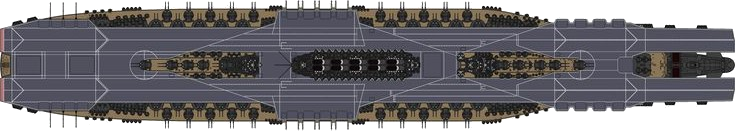
\includegraphics[width=\linewidth]{images/image BN V2/ship5.png}
      \caption{Bateau de taille 5}
      \endminipage\hfill
      \minipage{0.48\textwidth}
      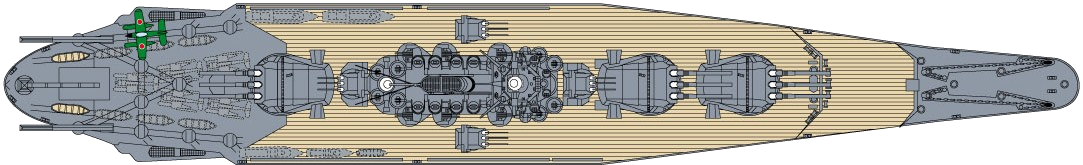
\includegraphics[width=\linewidth]{images/image BN V2/ship4.png}
      \caption{Bateau de taille 4}
      \endminipage\hfill
\end{figure}

\begin{figure}[H]
      \minipage{0.48\textwidth}
      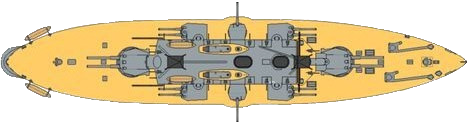
\includegraphics[width=\linewidth]{images/image BN V2/ship3.png}
      \caption{Bateau de taille 3}
      \endminipage\hfill
      \minipage{0.48\textwidth}
      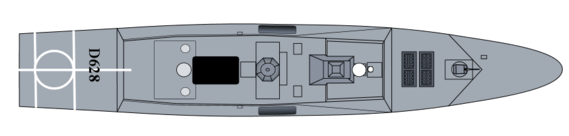
\includegraphics[width=\linewidth]{images/image BN V2/ship2.png}
      \caption{Bateau de taille 2}
      \endminipage\hfill
\end{figure}

\bigskip

Pour l'affichage du bateau on utilise une \textbf{ImageView}. C'est elle qui
est manipulée et c'est sur elle que la classe qui utilise un
\texttt{GraphicShip} met des écouteurs. Les méthodes de \texttt{GraphicShip}
sont des méthodes facilitant la manipulation comme:
\begin{minted}[bgcolor=lightgray, tabsize=2, fontsize=\small]{java}
      public void setSelected(boolean selected)

      public void setPlaced(boolean placed)

      public void rotate()
\end{minted}
\begin{itemize}
      \item[$\bullet$]\texttt{setSelected}: Permet de dire si le bateau est
      celui qui est manipulé.
      \item[$\bullet$]\texttt{setPlaced}: Permet de dire si le bateau est
      considéré comme placé.
      \item[$\bullet$]\texttt{rotate}: Permet de mettre le bateau à la
      verticale ou à l'horizontale.
\end{itemize}

\bigskip

\subsection{StartMenuAppli}
\begin{figure}[H]
      \centering
      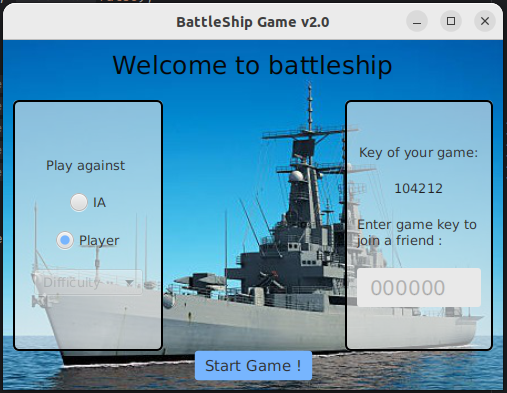
\includegraphics[width=0.60\linewidth]{images/image BN V2/startMenu.png}
      \caption{Écran de début de partie V2}
\end{figure}

Selon le mode de jeu choisi certaine partie de l'interface deviennent
inaccessible. Par exemple lorsque l'on sélectionne le mode JvJ on ne peut pas
choisir la difficulté de L'IA, car la \textbf{ComboBox} est désactivé. Le
\textbf{TextField} lui est soumis à un pattern matching basé sur l'expression
régulier suivante [0-9]{6}.

\bigskip

\subsection{ShipPlacer}
\begin{figure}[H]
      \centering
      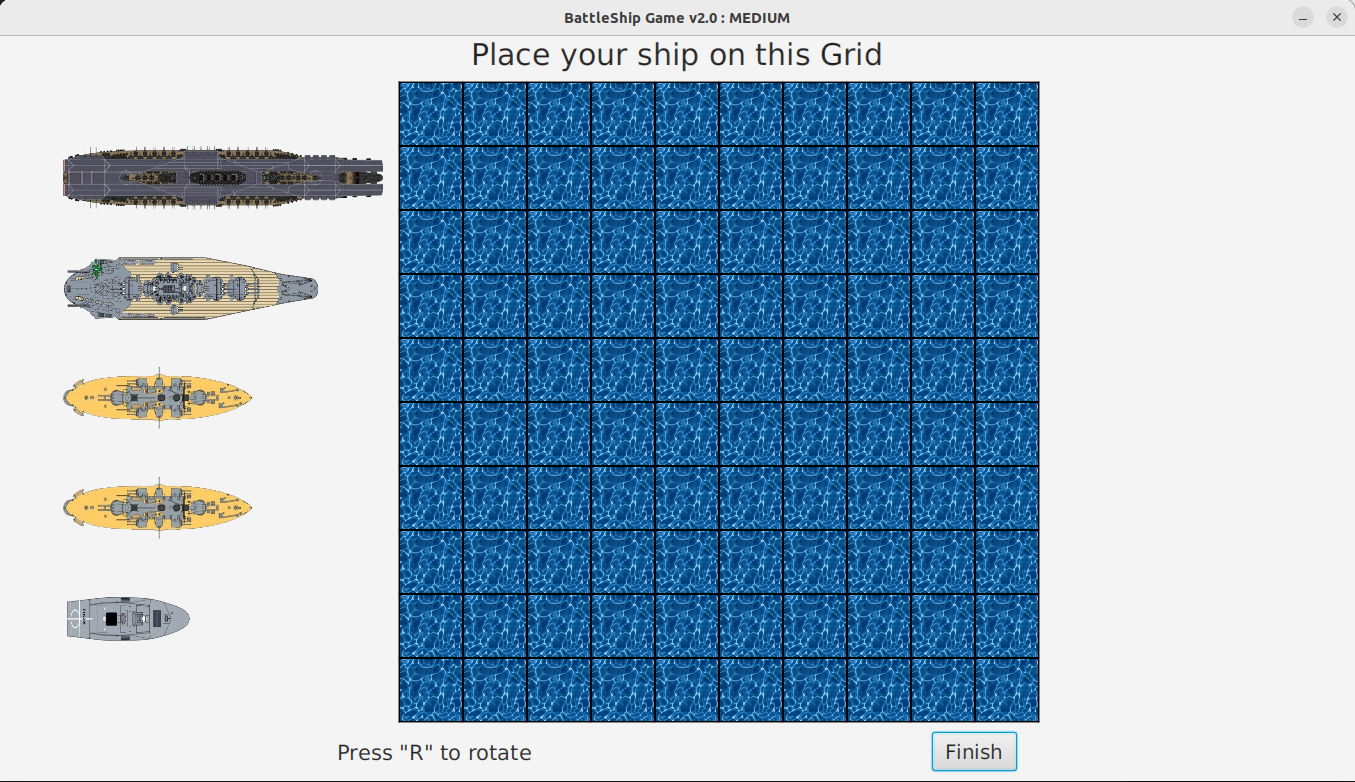
\includegraphics[width=\textwidth]{images/image BN V2/ShipPlacer.png}
      \caption{Écran de placement de bateau}
\end{figure}

La grille est une \texttt{GraphicGrid} et chaque bateau est un
\texttt{GraphicShip}. C'est la classe \texttt{ShipPlacerController} qui gère
l'ensemble des écouteurs des éléments de cette interface. Les coordonnées d'un
bateau sont calculées lors du relâchement de la souris. Si les coordonnées ne
sont pas valides alors le bateau est renvoyé sa position de base dans
l'interface. De même si le bateau est par-dessus un autre bateau déjà placé.

\bigskip

\subsection{Écran d'attente}

Si vous jouez contre un autre joueur et que vous êtes le premier à se connecter
à la partie vous verrez un écran d'attente jusqu'à ce que l'adversaire se
connecte.
\begin{figure}[H]
      \centering
      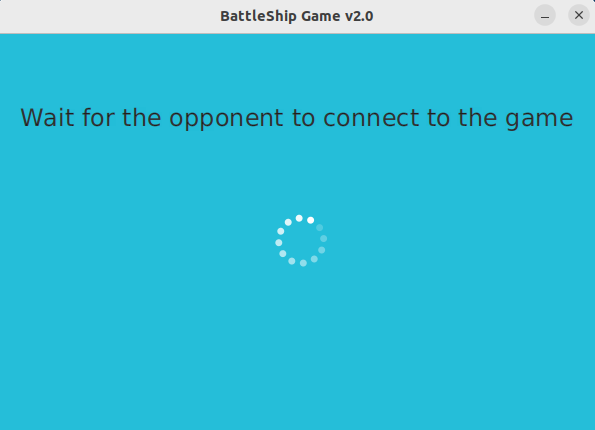
\includegraphics[width=0.60\textwidth]{images/image BN
            V2/waitingScreen.png}
      \caption{Écran d'attente}
\end{figure}

\subsection{InGameAppli}
\begin{figure}[H]
      \centering
      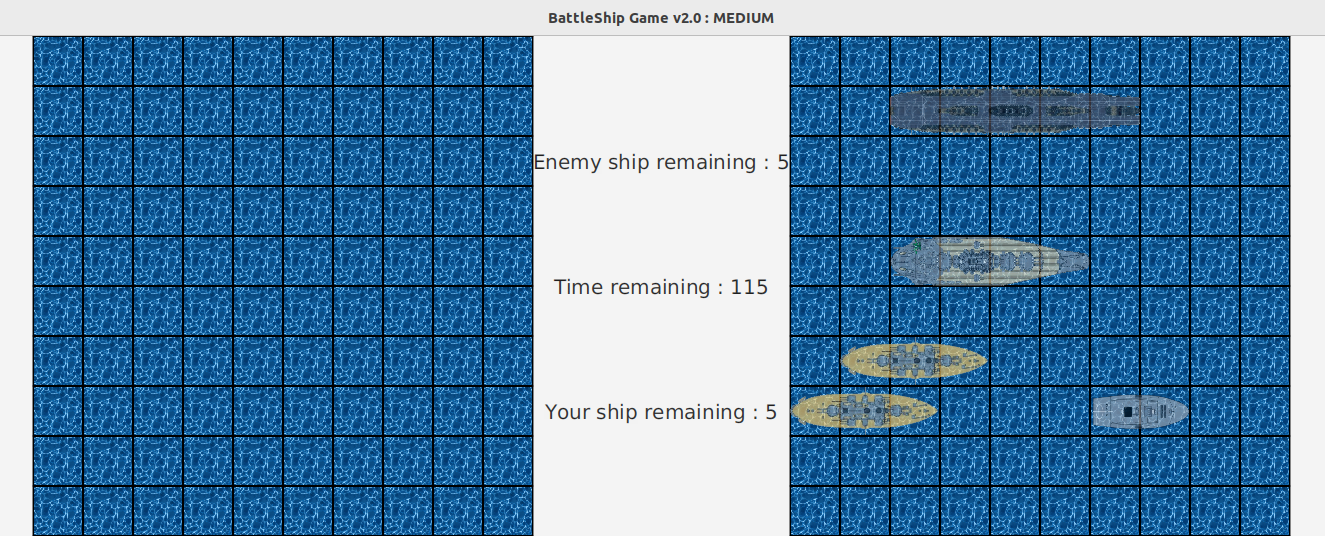
\includegraphics[width=\textwidth]{images/image BN V2/InGameAppli.png}
      \caption{Écran de partie}
\end{figure}

Les deux grilles sont des \texttt{GraphicGrid} et à des fins de confort de jeux
les bateaux fantômes représente l'emplacement des bateaux du joueur. Lorsque
c'est notre tour, on doit simplement cliquer sur la case que nous souhaitons
toucher. À noter que nous ne pouvons toucher deux fois la même case si nous
essayons cette pop-up apparaît.
\begin{figure}[H]
      \centering
      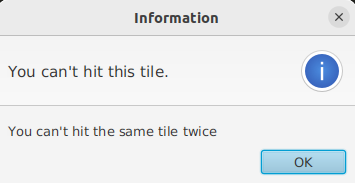
\includegraphics[width=0.48\textwidth]{images/image BN
            V2/DoubleTouche.png}
      \caption{Pop-up en cas de double touche au même endroit}
\end{figure}

\bigskip
Lorsque c'est le tour de l'adversaire, un effet grisé apparaît sur la grille et
aucune action dessus est possible.
\begin{figure}[H]
      \centering
      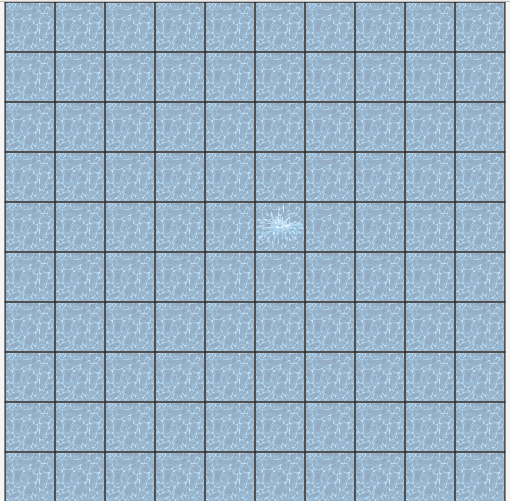
\includegraphics[width=0.48\textwidth]{images/image BN
            V2/OppenentTurn.png}
      \caption{Aspect de la grille de l'adversaire lors de son tour}
\end{figure}

\bigskip

La mise à jour des labels ainsi que des deux grilles se fait via l'écoute de
\textbf{PropertyChangeListener} sur les propriétés
\begin{itemize}
      \item[$\bullet$] \textbf{PROP\_TIMER} : Le temps restant pour le tour du
            joueur.
      \item[$\bullet$] \textbf{PROP\_ENEMY\_SHIP} : Le nombre de bateaux
            ennemis restant.
      \item[$\bullet$] \textbf{PROP\_SHIP} : Le nombre de bateaux restant au
            joueur.
      \item[$\bullet$] \textbf{PROP\_ENEMY\_GRID} : La grille de l'adversaire.
      \item[$\bullet$] \textbf{PROP\_GRID} : La grille du joueur.
\end{itemize}
\bigskip
D'autre \textbf{PropertyChangeListener} sont écoutés tels que
\begin{itemize}
      \item[$\bullet$] \textbf{PROP\_ROUND\_PLAYER} : Avoir connaissance si
            c'est le
            tour du joueur ou non.
      \item[$\bullet$] \textbf{PROP\_LOSE\_GAME} : Savoir si la partie est
            perdu.
      \item[$\bullet$] \textbf{PROP\_WIN\_GAME} : Savoir si la partie est
            gagnée.
\end{itemize}

\bigskip

\subsection{Écran de fin de partie}
\begin{figure}[H]
      \minipage{0.48\textwidth}
      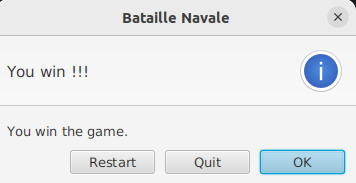
\includegraphics[width=\linewidth]{images/image BN V2/WinGame.png}
      \caption{Pop-up de fin en cas de victoire}
      \endminipage\hfill
      \minipage{0.48\textwidth}
      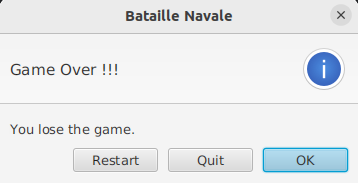
\includegraphics[width=\linewidth]{images/image BN V2/LoseGame.png}
      \caption{Pop-up de fin en cas de défaite}
      \endminipage\hfill
\end{figure}
Lors de la fin d'une partie on a le choix entre redémarrer une partie
\textbf{Restart}, ce qui nous amène vers l'écran de démarrage du jeu. Le bouton
\textbf{Quit} qui quitte l'application et le bouton \textbf{OK} qui
vas simplement fermer cette fenêtre tout en laissant l'interface de
\textbf{InGameAppli} inchangé.

\bigskip

\section{Annexe}
\subsection{Utilisation du programme}
\subsubsection{Programme Client}
\begin{itemize}
      \item [$\bullet$] Exécuter le fichier \texttt{launch.sh} dans le même
            répertoire que le fichier \texttt{keystore.jks}.
      \item [$\bullet$] Ou éxécuter cette commande:
            \begin{minted}[bgcolor=lightgray, tabsize=2, fontsize=\small]{bash}
      java --module-path ./javafx-path/lib 
      --add-modules javafx.controls,javafx.fxml,javafx.media 
      -jar BatailleNavale-1.0.jar
      \end{minted}
            Le jar doit être dans le même répertoire que le fichier
            \texttt{keystore.jks}.
\end{itemize}

\bigskip

\subsubsection{Programme Serveur}
\begin{itemize}
      \item [$\bullet$] Exécuter \texttt{java -jar ServerBatailleNavale.jar}
            dans un terminal dans le même
            répertoire que le fichier \texttt{keystore.jks}.
\end{itemize}

\bigskip

\subsubsection{Déroulement d'une partie en ligne}

Voici les étapes à suivre pour démarrer et jouer une partie contre un autre
joueur en réseau :

\begin{itemize}
      \item[$\bullet$] Dans l'écran de démarrage, cochez la case `Player', puis
            dans le champ de texte `key', rentrez un identifiant de partie (où
            laisser vide pour utiliser celui générer aléatoirement afficher
            au-dessus). Une fois fait, cliquez sur le bouton `Start Game' pour
            lancer la partie.
            \begin{figure}[H]
                  \centering
                  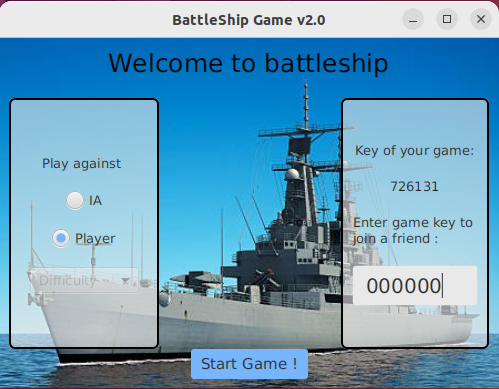
\includegraphics[width=0.48\textwidth]{images/image BN
                        V2/utilstart.png}
                  \caption{Utilisation du menu start contre un joueur}
            \end{figure}

            \bigskip
      \item[$\bullet$] Une fois sur l'écran de positionnement des bateaux,
            sélectionne un
            par un vos bateaux et placez-les sur la grille en maintenant le
            clique gauche
            enfoncée. Pour tourner le bateau un simple clic sur la touche `R'
            du clavier
            suffit.
            \begin{figure}[H]
                  \centering
                  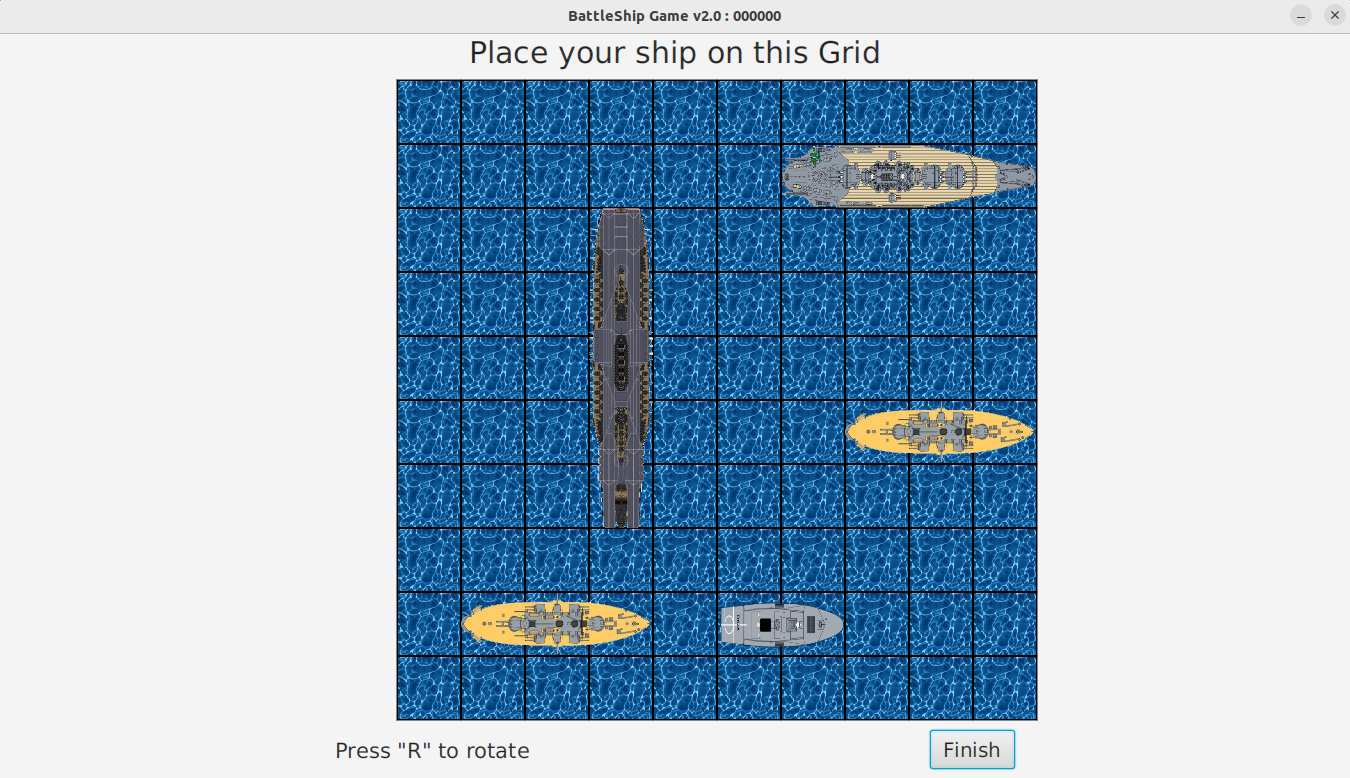
\includegraphics[width=\textwidth]{images/image BN
                        V2/utilshipplacer.png}
                  \caption{Utilisation de l'application de placement de bateau}
            \end{figure}
      \item[$\bullet$] Maintenant que tous vos bateaux sont positionnés,
            appuyez sur
            le bouton `Finish' pour passer à la suite.
      \item[$\bullet$] Vous pouvez maintenant jouer en tour par tour à la
            bataille
            navale, il suffit de cliquer sur la case que vous souhaitez
            toucher.
            \begin{figure}[h]
                  \centering
                  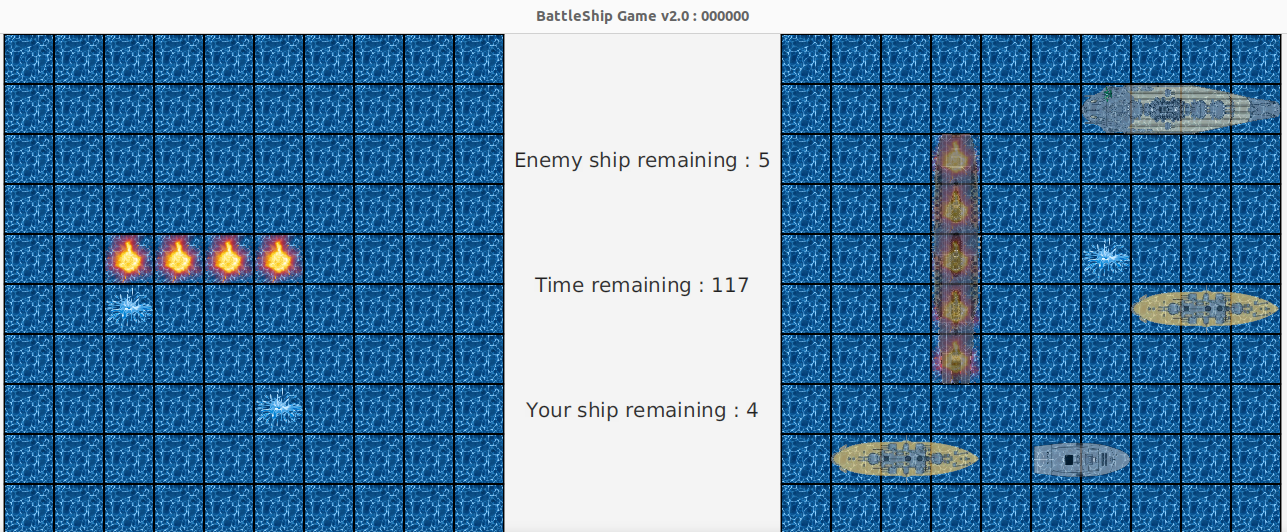
\includegraphics[width=\textwidth]{images/image BN
                        V2/utilsgame.png}
                  \caption{Utilisation de l'application de jeux}
            \end{figure}
      \item[$\bullet$] Une fenêtre apparaîtra dès que la partie sera terminée
            pour
            vous informer que vous avez gagné, perdu ou pire encore, que le
            serveur a eu un
            problème.
            \begin{figure}[H]
                  \centering
                  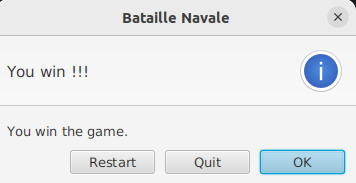
\includegraphics[width=0.48\textwidth]{images/image BN
                        V2/WinGame.png}
                  \caption{Exemple de fin de partie où le joueur gagne}
            \end{figure}
\end{itemize}

\subsection{Difficultés rencontrées}
\begin{itemize}
      \item[$\bullet$] La première difficulté que j'ai rencontrée et qui a duré
            toute la durer du projet est liée au fait que je découvrais JavaFX
            en même
            temps que je programmais ce qui à mener à passer beaucoup de temps
            à faire des
            recherches et aussi à beaucoup d'erreurs ou de parties non
            optimisées menant à
            des problèmes lorsque l'on veut modifier des parties ou régler des
            problèmes.
      \item[$\bullet$] La deuxième difficulté était sur l'interface graphique
            \texttt{ShipPlacer} pour la partie de `drag-and-drop' des bateaux,
            car il
            fallait que sur la grille les bateaux se déplace case par case et
            qu'on ne
            puisse pas mettre un bateau à moitié sur la grille et à moitié
            dehors, mais il
            fallait que tous, ces choses sois aussi respectés lorsque l'on
            tourne le
            bateau.
      \item[$\bullet$] La dernière difficulté est liée à la deuxième, c'est la
            gestion de la rotation des \texttt{GraphicShip} car la manière dont
            je l'ai
            fait ne permet pas une très grande liberté de manipulation, mais
            étant donné
            que c'est l'unique moyen que j'ai trouvé, c'est celui que j'ai
            adopté.
\end{itemize}

\subsection{Amélioration globale possible}
Des améliorations sur l'ensemble du projet possibles. En termes de
fonctionnalités données aux joueurs on peut penser à :
\begin{itemize}
      \item[$\bullet$] Le choix du nombre de bateaux : Cette fonctionnalité
            peut être introduite de plusieurs manières : Sois les joueurs
            choisis le nombre
            de chaque bateau ou avec une fonction qui génère automatiquement le
            bon nombre
            de chaque bateau en fonction du nombre total de bateaux. Les
            limites de cette
            fonctionnalité ont aussi plusieurs façons d'être introduites. Sois
            avec un
            nombre maximum défini en dur dans le code via une macroconstante ou
            avec une
            fonction qui calcule la totalité des cases occupées par les bateaux
            et si on
            peut donc placer l'ensemble des bateaux sur la grille.
            \bigskip
      \item[$\bullet$] GraphicShip: le composant graphique pour représenter les
            bateaux peut très sûrement être fait d'une autre manière permettant
            plus de
            liberté et limitant le nombre de problèmes pouvant être causé par
            la limitation
            de l'implémentation actuelle.
            \bigskip
\end{itemize}

\section{Conclusion}

Avoir retravaillé sur ce projet m'as permis de découvrir de nouvelles choses
telles que JavaFX et FXML\@. Ainsi que m'améliorer sur mon point faible, les
interfaces graphiques en Java. Je remercie mes camarades avec lesquelles j'ai
fait ce projet dans le cadre de l'Application Informatique, car j'ai pu
réutiliser les travaux ou m'en inspiré.

Je remercie également M. Guesnet pour ces conseils, avis et idées sur le
projet.

Je vous remercie d'avoir lu mon rapport, Leroy Florent.

\end{document}